\documentclass[11pt]{article}

\usepackage{algorithmic}
\usepackage{amsmath}
\usepackage{amsthm}
\usepackage{booktabs}
\usepackage{dcolumn} 
\usepackage{epstopdf}
\usepackage{fourier}
\usepackage{framed}
\usepackage{fullpage}
\usepackage[margin=1in]{geometry}
\usepackage{graphicx}
\usepackage{hyperref}
\usepackage{longtable} 
\usepackage{natbib}
\usepackage{rotating}
\usepackage{setspace}
\usepackage{silence}
\usepackage{tabularx}
\usepackage{verbatim}


% http://tex.stackexchange.com/questions/14938/plainnat-bst-without-natbib
\let\chapter\section
\usepackage[ruled]{algorithm2e}

\renewcommand{\algorithmcfname}{ALGORITHM}
\newtheorem{proposition}{Proposition}

 \onehalfspace
% \triplespace 
%\doublespacing 

%linespread{3}

\begin{document}

\title{The Allocation of Prominence on Two-Sided Platforms}

% \author{
%      JOHN J. HORTON 
%      \affil{oDesk Research}
%     JOHN GUNNAR CARLSSON 
%     \affil{University of Minnesota}
%     IOANNIS ANTONELLIS 
%     \affil{oDesk Research}
%     PANAGIOTIS PAPADIMITRIOU
%     \affil{oDesk Research}
%     GREG LITTLE 
%     \affil{oDesk Research}
%  }

% Todo 
% references to the equity criterion 
% replace visibility with prominence 
% Fix the latex sed thing 
% Move to importing create paper (.sh?)
% Add a TK punch list feature 

\maketitle

\begin{abstract} 
%%\ABSTRACT{
  We consider the problem two-sided platforms face in shaping the
  matches formed on the platform to reflect the platform's
  preferences. From this high-level motivation, we examine the problem
  in more concrete terms, using the main lever that platforms have for
  affecting matches---visibility of the trading parties to each
  other. We argue that the some of the standard ways of allocating
  visibility are likely to lead to allocations far away from what is
  efficient, given the platform creators preferences. We propose two
  mechanisms for shaping matches. The first is guaranteed to implement
  the platform's preferred, feasible allocation, but which is unlikely
  to be useful in practice due to its computational complexity. As an
  alternative, we propose a simple mechanism that reasonably
  approximates the first mechanism and is suitable for large scale
  application.
\end{abstract} 



\section{Introduction} 

In recent years, a number of electronic platforms that bring together
buyers an sellers have emerged. Examples include Apple's app store
(software, music, videos etc.), Amazon's seller network, eBay
(physical goods), and labor or expertise (oDesk, Innocentive, Elance,
99 Designs etc.). Prior research on two-sided platforms has focused
primarily on price structure and levels and competition between
platforms \citep{armstrong2006competition, rochet2003platform,
  rochet2006two, parker2005two}. This literature is largely descriptive, but it could
thought of as falling in the ``design economics'' literature
\citep{roth2002economist}, where price structure and levels are the
main instruments.

% While it 
% It is easy to show that under realistic assumptions that even under
% the guidance of a benevolent social planner, the 

%  The
% reason for this design focus is that the platform needs to impose some
% kind a price structure and level and these choices have implications
% for revenue.\footnote{The problem is analogous to the enormous
%   literature in public economics on optimal taxation}. We will show,
% using a simple but empirically grounded model that even if the
% platform was a benevolent social planner and had no need to impose
% fees of any kind, the ``natural'' outcome of interactions between
% buyers and sellers might not be welfare enhancing.

Despite the existing platform literature on price, we take the view
that price level and structure are not the only---and probably not he
most useful---instruments in the platform's ``toolkit.'' The reason is
that changing price structure and levels proves difficult in practice
once a marketplace has gained traction. Further, price is difficult to
experiment with, particularly when participants can easily compare
notes. \footnote{The recent Netflix pricing debacle is an example of
  the difficulty in making substantive price structure and level
  changes.} Furthermore, even if prices were easy to change, having a
simple price structure is often viewed as per se attractive from a
marketing perspective.

Given the limitations of price as a tool for platform design, what
other factors can platforms control that can shape platform
interactions in ways beneficial to the platform? We argue that one of
the most ``tune-able'' and powerful instruments in the platform
toolkit is the control of \emph{prominence} of users to each
other. Prominence directly affects the probability of matches forming,
since obviously parties that never see each other can never trade.

In traditional, non-electronic markets, buyers and sellers are
responsible for making themselves known to their would-be trading
partners. Gaining prominence might require as little effort as showing
up to trade at some specific time and place, or it might require a
massive advertising campaign. Regardless, the market's allocation of
prominence is de-centralized, arising from the decisions of many
individual actors.\footnote{There seems to be no consensus on the
  welfare properties of advertising. \cite{dixit1978advertising} argue
  that under a range of plausible assumptions, advertising is socially
  inefficient, though there are other works that take alternate views,
  claiming it depends on a number of factors
  \citep{becker1993simple}.}  By comparison, in electronic markets and
on electronic platforms, prominence is inherently determined by the
platform creators, as what is seen by users is set by the design
choices and policies of the platform. This power to control prominence
has not gone unnoticed or unexploited: the multi-billion dollar
position-based online advertising industry
\citep{varian2007position,edelman2005internet} is evidence for this
point.

Given the enormous literature on position auctions, one might be
tempted to think that the allocation of prominence is a solved
problem, with the solution being auctions. Although many platforms do
make use of auctions, they are far from universal and even when they
are used, often coexist with the unpaid ``organic'' display of
participants. There are numerous reasons why a platform might eschew
auctions but the general explanation is that platform member
preferences and willingness to pay do not perfectly align with
platform's preferences: the platform might worry that those choosing
to pay for position might be adversely selected, or the platform might
want to secure some minimal level of prominence for all users, to
ensure their continued participation and thus sufficient market
liquidity.  Even the existing of an explicit pay-for-prominence scheme
might undermine the credibility and thus the usefulness of the
platform as a whole.\footnote{An historic example is the legal
  prohibition on ``Payola,'' or the practice of record companies
  paying DJ's to play certain songs.} 

% TK transaction costs of auctions 

% We can now describe 

\subsection{Overview of the paper} 
In this paper, we consider the problem on a platform creator that has
some preference over the matches formed on the platform and that these
preferences will be acted upon by the platform allocating individuals
some ``share'' of prominence in the marketplace. To motivate the
problem, we first present a very simple model of platform dynamics
that will show how a situation in which all participants have full
knowledge all participants (i.e., prominence is irrelevant) is not
socially optimal. We will show that this situation can be improved by
restricting prominence. In the model, market failure arises from too
much attention being focused on platform ``veteran'' sellers, with too
little discovery of novice sellers---a problem known to be important
in several marketplaces.

The focus of the paper will shift to solving the problem in the form
it is most likely to take in practice---allocating individuals to some
number of ``slots,'' each which afford the occupant of that slot some
share the of ``prominence'' which is attention from would-be buyers
and can be thought of in practice as page views or impressions. We
will assume that attention comes from buyers and that sellers are the
ones being allocated prominence, though in reality, search could be
conducted by buyers, sellers or both. Platform preferences for seller
prominence are modeled as a ``budget'' for each seller, which is the
share of the available prominence that the seller should receive in
expectation. We will assume that the attention itself is homogeneous,
i.e., we will not draw distinctions between which buyer is generating
the attention.

We will show by example that seemingly reasonable strategies for
allocating sellers to slots (such as always rank ordering sellers by
some notion of merit like feedback scores) leads to highly unequal
allocations of prominence that are likely to be far away from the
platform's preferences. Furthermore, these simple allocation
mechanisms lack desirable properties like continuity (which can cause
sellers with only slight differences receiving radically different
amounts of attention on the platform). Using data from an actual
two-sided platform, where we have measures of prominence and
congestion, we will show that the buyer attention to different
``slots'' (position in search results) follow a Zipfian distribution
and that unless the platform's preferences for the allocation of
prominence to sellers also follows the precise Zipfian distribution of
attention shown to the slots.

In this framework, the allocation of individuals to slots becomes an
economic assignment problem. We review the existing literature on
these mechanisms and propose two mechanisms of our own. The first
mechanism is guaranteed to give allocations of prominence consistent
with the platform's preferences (as captured by the sellers
budgets). It works by solving an linear program. Unfortunately, it is
impractical, having a computational complexity of $\mathcal{O}(n^5)$,
making in unsuitable for the large-scale two-sided platforms
motivating the problem.

As an alternative, we propose a substitute which we call the ``reverse
tontine'' (RT) mechanism. While it does not guarantee that prominence
allocations are consistent with seller budgets, it does offer
continuity and monotonicity in budgets with respect to the expected
prominence allocation. Furthermore, the distribution of prominence
allocations under RT for a higher budget seller first-order
stochastically dominates the outcomes for a lower budget seller,
ensuring that a rational seller will always prefer to have a higher
budget. Simulation studies using parameters from an online labor
market show that the RT does quite well in implementing the platform's
preferences. As a practical matter, we show that RT allocations can be
generated very quickly and has limited memory requirements. It is also
easy to update with changed budgets and changes in the prominence
associated with different slots, making it suitable for application on
platforms with large numbers of participants.



%\documentclass[11pt]{article}

\usepackage{booktabs}
\usepackage{colortbl}
\usepackage{dcolumn} 
\usepackage{epstopdf}
\usepackage{fourier}
\usepackage{fullpage}
\usepackage{graphicx}
\usepackage{hyperref}
\usepackage{longtable} 
\usepackage{natbib}
\usepackage{rotating}
\usepackage{setspace} 
\usepackage{Sweave} 
\usepackage{tabularx}

\hypersetup{
  colorlinks,
  citecolor=blue,
  linkcolor=blue,
  urlcolor=blue,
  filecolor=white
}

\newtheorem{proposition}{Proposition}

\title{Here is a title}

\begin{document}
   \maketitle



 

\section{Platform's design challenge} 
Different platforms have different preferences of the matching of
platform participants. These preferences presumably differ over
time. For example, a nascent platform is probably more worried about
market liquidity and growth, where as an established platform, focuses
more on revenue, cost and retention. It is beyond the scope of this
paper map various macro-level platform preferences to different
strategies implemented via budgets for sellers. However, it is still
useful to (a) characterize a common platform problem and (b) show how
it is addressable via the controlled allocation of prominence.

A common problem in electronic markets where quality is a factor is
that novices---those without a market reputation---have difficulty in
finding a trading partner and/or must sell a discount. For example,
\cite{resnick2006value} found that new sellers without an eBay
reputation ended up selling identical goods at an 8\% discount
compared to veteran seller. This problem is perhaps more acute in
labor markets, where uncertainty about seller quality and reputation
is greater and potentially more important. 

\cite{tervio2009superstars} develops a model of a labor market in
which hiring firms focus too much attention on veterans and not enough
on ``talent discovery'' i.e., the hiring of novices. The gist of the
model is that talent discovered via hiring becomes common knowledge
post-hire, and since workers are not obligated to stay with their
hiring firm, hiring firms cannot fully recoup the costs of talent
discovery. \cite{pallais2010inefficient} tested this model on oDesk
with an experiment in which she hired a treatment group of 952 workers
for a task and gave them public feedback for their work.  The control
group received no job (and hence no feedback). Most of the workers in
the experiment had no experience on the platform. Pallais finds that
her treated group of workers were able to substantially raise their
earnings once equipped with a reputation. In fact, the workers were
able to earn more from other buyers than the total cost of the
experiment with a few months.

The theoretical results from Tervi{\"o} and empirical results from
Pallais imply a clear challenge for platform creators, which is to
push more firms to hire novices. In the model below, we will assume
that the platform simply wants to maximize total social surplus. A
for-profit platform actually has different incentives depending on
price structure (for example, a platform that charges a fixed
percentage will want to maximize the NPV of the wage bill), but for
illustrative purposes, these complications are not relevant.

% Novices---those without feedback or reputations---often have great
% difficulty getting started in markets (TK - cite Zeckhauser). Online
% labor markets are known to suffer this problem to an extreme degree
% (TK - cite Pallais, Tervio, Stanton). In the Tervio model, The root of
% the problem is that talent discovery is inefficiently under-supplied
% in the marketplace, at least in part because workers cannot subsidize
% their own discovery.
 
% \subsection{Match probability as mediated by platform creators}

% \subsection{Price level and structure---carved in stone?} 

% When a platform entirely forgoes prices, prominence is still
% allocated, but the allocation depends on some other criteria set by
% the platform, such as lexical ordering, recent activity, chronology
% etc. 

% For example, craigslist orders results within
% categories by time of posting, as does Amazon Mechanical Turk
% (MTurk).\footnote{Not surprisingly, this time-based ordering leads to
%   manipulation as participants try to increasing their prominence. See
%   \cite{chilton2010task} for a discussion of this phenomena on MTurk.}
% On other sites, returned results are often ordered based on some
% algorithmic notion of relevancy, such as tf-idf or PageRank
% \cite{page1999pagerank}.

\subsection{Platform growth and talent discovery} 
Consider a marketplace with a fixed pool of buyers with measure
$1$. We will assume that the sellers are selling labor and that a
buyer choosing to purchase labor from a particular seller can be
thought of as hiring that seller. There are two types of sellers:
those that are good, and produce an output of $1$ if hired, and bad,
that produce nothing if hired. The proportion of good sellers is
$\theta$ and the measure of sellers if $\theta^{-1}$.

All sellers start as \emph{novices}. When a seller is hired, their
type is revealed publicly to the marketplace. Bad sellers exit the
marketplace, while good workers become \emph{veterans}. We will assume
that all parties are price takers and that wages are $w_V$ for
veterans and $w_N$ for novices, with $\theta < w_N < w_V < 1$ and $1-
w_v > \theta - w_n$. This ensures that firms would rather hire a
veteran than a novice, but they would rather hire a novice that not
hire anyone at all.

For any discount rate, the platform wants (a) all veterans to matched
with buyers, to get the guaranteed payoff this promises) and (b) all
other buyers hiring novices, in order to turn some fraction into
veterans. If matching occurs in continuous time and $v(t)$ is the
number of veterans in the marketplace, the socially optimal evolution
of the marketplace will be:
\begin{equation}
v_{0}'(t) = (1-v_0(t))\theta
\end{equation}
with $v_0(0)=0$, which has the solution of $v_0(t) = 1-e^{-\theta
  t}$. However, if the platform cannot fully control the matches that
are formed, we can have a situation where multiple buyers compete for
the services of the same veteran, even though only one match is
possible. We will assume that veterans pick randomly from the pool of
buyers courting them. Further, we will assume that buyers can sort
themselves such that they can obtain the best possible terms (i.e.,
all veterans will receive the same number of applicants, in contrast
to a ball-and-urn model of applications where the realized number is
binomial random variable).

Let us not assume that a fraction $r$ of buyers will pair with novices
and $1-r$ with veterans. We will indicate the measure of veterans at
time $t$ as $v_1(t)$. This makes $v_1'(t) = r\theta$. At time $t$, the
probability that buyer seeking the services of a veteran will be
successful is $v(t) (1-r)^{-1}$. In equilibrium, the returns to
seeking out a veteran have to be equal to seeking out a novice, hence
$\theta - w_n = v_1(t)(1-r)^{-1} (1 - w_v)$ so $r = 1 - (1 -
  w_v)(\theta - w_n)^{-1}v(t)$, and hence: 
\begin{equation}
  v_1'(t) = \left(1 - \frac{1 - w_v}{\theta - w_n}v_1(t)\right)\theta 
\end{equation} 
Since $1 - w_v > \theta - w_n$, we know that $v_1'(t) < v_0'(t)$---the
supply of veterans grows more slowly in the unorganized market where
buyers are allowed to compete for the scarce pool of veterans. Not
only is growth slower, it eventually stalls completely once $\theta -
w_N = v_1(t)(1-w_v)$. This ``stalling'' of the marketplace occurs once
the number of veterans reaches $\underline{v} = (\theta - w_n)(1
  - w_v)^{-1}$. Once the platform reaches $\underline{v}$, the
talent-discovery stops and no novices every get hired: buyers are
content to take their chances with the over-subscribed veterans. The
expression for $\underline{v}$ offers intuitive comparative statics:
the lower the baseline level of talent, lower the $\theta$, the more
rapidly the marketplace stalls. Higher wages for novices has a
similarly stifling effect, as does low wages for veterans.

\subsection{Tilting the marketplace towards optimal growth}
If the platform wanted to continue to grow at the optimal rate, it
could divert the excess buyer attention away from the veterans and
towards the buyers. To formalize this intuition, let us imagine that
we are allocating the buyer attention (which as the same measure as
the buyers, i.e., $1$) amongst the veterans the novices. We can think
of this allocation as a ``budget'' we give to a veteran $b_v$ and a
budget given to a novice, $b_n$.

To obtain the optimal growth path for the platform, we need to
allocate $v(t)$ of the attention to the veterans and $1-v(t)$ to the
novices. The number of novice sellers at time $t$ is $\theta^{-1} -
v(t)\left(1 - \theta^{-1}\right)$, and so
\begin{eqnarray}
b_v &=& v(t) \nonumber\\
b_n &=& \frac{1-v(t)}{\theta^{-1} - v(t)\left(1 - \theta^{-1}\right)}
\end{eqnarray} 

\subsection{Static example with heterogeneous match probabilities}
To give an example of the usefulness of this prominence budget
conception, let us consider a platform that is no longer growing but
simply wants to maximize the number of matches formed. Unlike in the
simplified example before, let us more realistically assume that each
seller $i$ has some exogenous match probability $q_i$ when exposed to
a single buyer. As we assumed previously, sellers have limited
capacity and thus can form at most one match. This means that for any
seller, there are decreasing returns to attention by buyers. Let $b_i$
be the number of ``impressions'', allocated to a seller. The total
amount of impressions is $A$ (for attention).

The probability that a seller fails to form a match when given one
unit of impressions is $1-q_i$. The probability of forming no matches
when giving $b$ units of visibility is $(1-q_i)^b$ and thus the
probability of forming a match (and nice approximation to this
probability) is:
\begin{equation} 
m_i(b) = 1 - (1 - q_i)^{b} \approx 1 - e^{-q_i b}
\end{equation} 
The platform now faces a constrained optimization problem:  
\begin{equation}
\max_{\vec{b}} \quad L = \sum_i \left(1 - e^{-q_i b_i}\right) + \lambda \left(A - \sum b_i\right) 
\end{equation} 
The first order condition is $q_i e^{-q_i b_i} - \lambda \ge 0$. The
shadow value of the constraint is $\lambda$, which can be thought of
the additional matches possible from one additional unit of attention
to distribute. At the optimum, each seller either (a) offers the same
marginal probability of forming a match or (b) gets no attention at
all. We can re-formulate the FOC as a linear equation $-q_i b_i + \log
\lambda (q_i)^{-1} = 0$ conditional upon $a_i > 0$. 

First let us consider the $n=2$ case and assume that there is an
interior solution, i.e., $b_1 > 0$ and $b_2 > 0$. The first order
conditions are:
\begin{eqnarray}
q_1 e^{-b_1q_1} + \lambda &=& 0 \nonumber\\
q_2 e^{-b_2q_2} + \lambda &=& 0 \nonumber\\
b_1 + b_2 = A 
\end{eqnarray} 
which we can re-write as 
\begin{eqnarray}
-b_1q_1 + b_2q_2  &=& \log \frac{q_2}{q_1} \nonumber\\
b_1 + b_2 & = & A 
\end{eqnarray} 
which is a system of linear equations. To ease explication in the $n >
2$ case, we will write this system in matrix notation. 
\begin{equation}
\left( \begin{array}{cc}
-q_1 & q_2  \\
1 & 1  \end{array} \right) 
\left( \begin{array}{c}
b_1   \\
b_2    \end{array} \right)
=
\left( \begin{array}{c}
\log \frac{q_2}{q_1}   \\
A    \end{array} \right)
\end{equation} 

Let us now consider the $n > 2$ case. The matrix equation is the
standard equation for a system of linear equations: $M \vec{b} =
\Gamma$. We can define the entries of $M$ as:  
\begin{equation}
\mu_{ij} =
\begin{cases}
-q_i, & \text{if }i = j \wedge j \ne n \\
q_{i+1}, & \text{if }i + 1 = j \wedge j \ne n \\ 
1, & \text{else} 
\end{cases}
\end{equation}
Note that the last row contains all $1$'s---this is just the
constraint that the sum of all allocations equals the attention
available. To construct the column vector $\Gamma$, we can use the
same simplification of dividing the $i$th equation by the $i + 1$th
equation to create:
\begin{equation}
\gamma_{i} = 
\begin{cases}
\log \frac{q_{i+1}}{q_{i}}, & \text{if }i < n \\
A, & \text{if }j = n \\ 
\end{cases}
\end{equation}
We have a system of linear equations that we can solve.  
\begin{equation} 
[ m_{ij} ] \vec{b} = [ \gamma_i ]
\end{equation} 

\paragraph{Finding interior solutions}
Not all sellers will get attention in this formulation: if $q_k <
\lambda^*$ (i.e., the marginal benefit from a seller when $a=0$ is
less than the shadow value of the constraint at the optimum), the
seller is excluded. One complication in the linear system approach
outlined above is that solving the system does not exclude these
sellers (they receive negative weight). Further, we cannot simply find
the first negative weight seller and draw the cut-off there: the
cutoff depends on the shadow value estimated with the proper set of
workers. 

A heuristic for solving the problem is to use a binary search to
identify the smallest-q sellers that still receives positive attention
the optimal solution, operating on list of sellers, sorted from
highest to lowest value. This does require solving the system of
linear equations at each step, though the speed of binary search
(combined with some probably places for optimization) does not make
this intractable.  

% k = p_1 e^{p_1 x_1} =  p_2 e^{p_2 x_2} = p_3 e^{p_3 x_3}
% ln(p_1) + p1*x1
% Without coming up with an actual budget for each seller, 

% The platform creator wants to make sure that of the buyer's searches,
% a fraction $v$ ending up on veterans, and a fraction $1-v$ end up on 
% novices.  

%\end{document}


\subsection{Applied allocation of prominence}
In the previous example, we talk about allocating prominence as if it
were something that could be apportioned out by the platform by fiat,
in whatever fine-grained distribution required. In reality, prominence
on a platform is mediated by page position/rank order in returned
search results, with each position offering some flow of page views
and clicks (i.e., prominence). This means that prominence comes in
``lumps'' that differ (often dramatically) in size, with the
distribution of lump sizes seeming to follow familiar patterns across
sites. What this means in practice is that turning platform
preferences into prominence budgets is not sufficient: we need some
mapping from these budgets to actual positions.

Let us assume that we have $n$ individuals that we need to assign to
$n$ slots. Each of the $n$ positions has a ``value'' $v$ (i.e., an
associated visibility) such that $v_1 > v_2 > v_3 \ldots v_n$. In this
paper, we will be concerned solely with stochastic assignment
mechanisms, i.e., a mechanisms that will place an individual $i$ at
position $j$ with probability $p_{ij}$. We evaluate allocations based
on the expected values they generate for an individual $i$, which we
will call $x^n_i = \sum_{j=1}^n p_{ij}v_j$, as well as the
distributional properties of the allocation mechanism.



\section{Allocation mechanisms}
The allocation of prominence on a platform has clear analogies to the
economic allocation problem, in that the platform has a number of
slots that differ in their value and a number of items---people,
websites, advertisements, etc.---that must be assigned to a slot. The
economic literature on making these kinds of allocations in the
absence of a price mechanism goes back to
\cite{hylland1979efficient}. In the setting Hylland-Zeckhauser
formulation, individuals have cardinal preferences, which they use to
``buy'' probability shares, giving a bistochastic matrix which can be
used to generate allocations.

Subsequent work on the assignment problem has focused on cases where
only ordinal preferences are known, with the literature presenting
various mechanisms and evaluating their efficiency and
strategy-proofness (or lack thereof)
\citep{kojima2010incentives,manea2007serial,abdulkadiroglu1999house}. The
two main solutions in the literature are the serial dictatorship and
the probabilistic serial mechanism.\footnote{In the probabilistic
  serial mechanism proposed by \cite{bogomolnaia2001new}, every
  individual simultaneously ``eats'' unit probability shares at a
  constant, common rate, with each individual starting at their
  preferred position. When an individual's current position is totally
  consumed, they move to their next best option until time runs
  out. \cite{budish2009implementing} gives a procedure for drawing
  allocations from the resultant bistochastic matrix.}  In the serial
dictatorship, individuals are ranked according to some criterion
(possibly randomly ranked); the first-ranked individual gets their
first choice, the second gets to pick from what is remaining, and so
on until all choices are exhausted. This is actually the only
mechanism that is fair and efficient, in the sense that a
higher-ranked individual would never envy a lower-ranked individual
\cite{balinski1999tale}.

While the economic assignment problem provides a framework, allocating
prominence on platforms has a number of important distinguishing
features. One important difference is that on a platform, we expect to
re-allocate individuals to slots continually, perhaps even in response
to every new query by a buyer. In contrast, the economic literature
was motivated by one-off scenarios such as the assigment of students
to schools, families to houses, kidneys to patients, etc. As such,
there is a natural focus in economics on the equity of the single
realized allocation. In the platform case, we are must more interested
in expectations and the distributional properties of assignment
mechanisms.

In a one-shot ``ecnonomic'' scenario, the simple serial dictatorship
is an appealing solution, but if done repeatedly, with the same set of
choices and the same set of individuals, it can easily run afoul of
the common-sense notion that equals should be treated equally. To see
the problem, suppose there are two individuals with budgets $b_1 =
0.8$ and $b_2 = 0.2$ that must be assigned to two positions that offer
value (i.e., visibility) worth $v_1 = 80$ and $v_2 = 20$. The simple
serial dictatorship is the only obviously fair solution: the higher
budget individual gets the higher value position. Further, the
benefits are proportional to relative budgets. However, as either the
ratio of budgets or ratio of position values change, the obviousness
fairness of the simple serial dictatorship wanes: the higher budget
person still gets the higher value position, but proportionality is
lost. And no matter how close the two individuals become in budgets,
gap between their expected payoff does not diminish. Even when $b_1 =
1 + \epsilon$ and $b_2 = 1$, individual $1$ gets a (proportionally
speaking) windfall of $30$ and individual $2$ loses $50$, no matter
how small $\epsilon$.

Intuitively, as $\epsilon$ gets smaller, the two individuals should
each get $v_1$ and $v_2$ in approximately equal proportion. This of
course means that sometimes the strictly lower-merit individual gets
the top position, sacrificing fairness in one realization for a gain
of fairness in expectation. We want the mechanism to capture the
notion that likes should be treated alike, which in this case means
that expected value is continuous in merit. Further, expected value
should also be monotonically non-decreasing in merit (i.e., an
individual should never wish they had a smaller budget).

% the
% motivation for this paper---the allocation of prominence on two-sided
% platforms---has properties that make the standard economic approaches
% unattractive. One difference is that the economic literature is
% generally focused on cases where all individuals should be treated
% equally, whereas platforms almost always want to give more visibility
% to some select participants.


% Each individuals has ``merit'' $b$, creating a
% vector of budgets, $\vec{b}$.  

% This formalization immediately highlights another important
% difference between this setting the common economic allocation
% setting: notice that the values associated with positions are not
% conditional, i.e., we are assuming that all individuals have identical
% ordinal preferences, with everyone preferring more visibility to
% less. As such, the serial dictatorship and the probabilistic
% dictatorship give identical results.\footnote{To see why, consider
%   that in the probabilistic serial mechanism case, all $n$ individuals
%   would start ``eating'' probability at the most valued position
%   (since this is every individual's first choice). Each would be able
%   to eat $1/n$ and then, all at once, all would move to position 2,
%   where they would eat $1/n$, and so on. The resultant bistochastic
%   matrix is identical to that generated by the serial dictatorship.}

% Another important difference between the classic economic allocation
% scenario and our setting is that the economic literature was motivated
% by one-off scenarios such as the assigment of students to schools,
% families to houses, kidneys to patients, etc. As such, there is a
% natural focus on the equity of the single realized allocation. In
% contrast, on platforms individuals can be re-allocated many hundreds
% of times per day, appearing in different orders in response to
% different queries. As such, expected visibility and the properties of
% the distributio of realized outcomes becomes more interesting and more
% important.  A final difference that is common to many (but not all)
% two-sided platforms is that the limited capacity of the platform
% participants suggests that frequent changes in ``merit'' should be
% made, so as to make sure the same over-exposed individuals do not
% continually appear at the top of the search results.

% \subsection{Practical importance of justice}
% Within two-sided platforms, the ``thing'' being allocated visibility
% is often not a website or a product but a person.  This is a
% non-trivial difference, as it gives a technical resource allocation
% problem an ethical dimension and as such, any choice by the platform
% creator is likely to generate strong emotions. Whether they perceive
% it that way or not, the platform creator is implicitely assigning
% visibility according to some notion of justice. This is likely to
% prove contentious. Aristotle wrote in Book V of his Nichomachean
% Ethics:
% \begin{quote}
%   [T]his is the origin of quarrels and complaints---when either equals
%   have and are awarded unequal shares, or unequals equal
%   shares. Further, this is plain from the fact that awards should be
%   ``according to merit''; for all men agree that what is just in
%   distribution must be according to merit in some sense, though they
%   do not all specify the same sort of merit...
% \end{quote} 
% We can easily achieve Aristotle's ideal when goods are divisible, but
% the problem becomes more challenging when goods (or ``bads'') are
% indivisible, e.g., jobs, unpleasant duties, artwork, custody of
% children, etc. An ancient solution to this dilemma is to introduce some
% randomization device like drawing lots.

% Pure randomization works well when all should be treated equally, but
% what if individuals are unequal? It then no longer seems fair to
% allocate by a lottery that treats individuals exactly the same (a
% point made by Aristotle). 


% \subsection{Rivalrousness and the need for frequent re-allocation} 
% TK - Make much shorter. 

% In situations where search is returning information (e.g., websites,
% documents, etc.), there is no inherent problem with returning the same
% result to every user in response to the same query. This relatively
% static approach (with updates only made to reflect improved estimates
% of relevancy) works because the returned results are non-rivalrous
% goods: the effect of the marginal visitor on the remaining visitors is
% effectively zero, which means that every visitor can be shown the
% ``best'' page without that page being consumed. While this
% non-rivalrousness is true of web pages, it is not true for many other
% things that might be returned from search, such as individual buyers
% and sellers.

% Rivalrousness becomes an issue when the returned results have limited
% capacity, which is characteristic of many two-sided platforms (e.g.,
% most individuals can only work 40 to 50 hours per week, go on so many
% dates, knit so many custom sweaters, etc.). The issue is that
% visibility in search tends to follow a power law distribution, with
% the top results getting a large fraction of the views and hence
% contacts by would-be buyers or sellers. The fire hose of attention can
% quickly exhaust the capacity of those on top. In short order, the the
% individuals getting the most visibility need it the least and
% searchers are quickly discouraged by the low response rate to their
% contacts. This characteristic makes it critical for applied purposes
% that budgets can be updated in nearly real-time.

\subsection{Exact solution} 
In this section we show how to determine a collection of $n\times n$
permutation matrices $\Pi_{k}$, together with a collection of
probabilities $\alpha_{k}$, such that the marginal probabilities
$p_{ij}$ induced by the $\Pi_{k}$'s and the $\alpha_{k}$'s (that is,
$p_{ij}=\sum_{k}\alpha_{k}\pi_{ij}^{k}$, where $\pi_{ij}^{k}$ denotes
the $ij$th element of the matrix $\Pi_{k}$) satisfy the exact
proportion criterion \[
\frac{b_{i}}{\sum_{j}b_{j}}=\frac{\sum_{j}p_{ij}v_{j}}{\sum_{j}v_{j}}\,\]
If no such collection exists (which we can also verify), we give a
collection of permutation matrices whose ``distance'' from the exact
proportion criterion is minimized in the least-squares sense, i.e. we
find marginal probabilities $p_{ij}$ that minimize\[
\sum_{i}\left\Vert
  \frac{b_{i}}{\sum_{j}b_{j}}-\frac{\sum_{j}p_{ij}v_{j}}{\sum_{j}v_{j}}\right\Vert
^{2}\,\] To simplify notation, we suppose without loss of generality
that $\sum_{i}b_{i}=\sum_{j}v_{j}=1$ and therefore our exact
proportion condition is merely that $b_{i}=\sum_{j}p_{ij}v_{j}$ for
all $i$. It is obvious that the matrix of marginal probabilities, $P$,
should be the solution to the least-squares problem\[
\mathrm{minimize}_{P}\left\Vert Pv-b\right\Vert _{2}^{2}\] which is
easily solved using standard convex optimization methods (if desired
one could also consider minimizing $\left\Vert Pv-b\right\Vert _{1}$
or $\left\Vert Pv-b\right\Vert _{\infty}$, which can be done using
linear programming). The optimal objective function value to the above
problem is $0$ precisely when $P$ satisfies the criterion.

Let $P^{*}$ denote the optimal solution to the least-squares problem;
we now consider the problem of determining a collection of permutation
matrices $\Pi_{1},\dots,\Pi_{K}$ and positive scalars
$\alpha_{1},\dots,\alpha_{K}$ such that the marginal probabilities
induced by the $\Pi_{k}$'s are precisely the matrix $P^{*}$, i.e. that
$p_{ij}^{*}=\sum_{k}\alpha_{k}\pi_{ij}^{k}$ for all $i,j$. This is a
straightforward application of a theorem of Birkhoff
\cite{marcus}. The main idea is that if we are given an $n\times n$
doubly stochastic matrix $P$, there must exist an $n\times n$
permutation matrix $\Pi$ such that $\pi_{ij}=1$ implies that
$p_{ij}>0$ (i.e. $\Pi$ only has $1$'s in entries whose corresponding
value in $P$ is nonzero). If this is the case, we let $t$ be the
minimum value of $P$ whose corresponding entry in $\Pi$ is $1$,
i.e. \[ t=\min_{i,j:\pi_{ij}=1}p_{ij}\,\] Clearly if $t=1$ then $P$ is
a permutation matrix. If $t<1$ then the matrix $(1-t)^{-1}(P-t\Pi)$
has one fewer nonzero entry than $P$. We then perform this procedure
recursively on the elements of $P$ (at most $(n-1)^{2}$ times) until
$t=1$ and we are done; see Algorithm \ref{alg:find-equitable}.  Since
Algorithm \ref{alg:find-equitable} requires that we solve a bipartite
matching problem $\mathcal{O}(n^2)$ times, and since the Hungarian
algorithm requires $\mathcal{O}(n^3)$ running time
\citep{burkard2009assignment}, the overall complexity of Algorithm
\ref{alg:find-equitable} is $\mathcal{O}(n^5)$.

\begin{algorithm}
\caption{Exact Proportion (EP). This algorithm takes as input a pair
  of nonnegative $n$-vectors $b$ and $v$ such that
  $\sum_{i}b_{i}=\sum_{j}v_{j}=1$ and outputs an $n\times n$ marginal
  probability matrix $P^{*}$ that minimizes $\left\Vert
  Pv-b\right\Vert _{2}^{2}$, as well as a collection
  $\mathtt{Permutations}$ of at most $(n-1)^{2}$ permutation matrices
  $\Pi_{k}$ and associated probabilities $\alpha_{k}$ such that
  $P^{*}$ is the marginal probability matrix of the $\Pi_{k}$'s and
  the $\alpha_{k}$'s, i.e. $p_{ij}^{*}=\sum_{k}\alpha_{k}\pi_{ij}^{k}$
  for all $i,j$.  }
\label{alg:find-equitable}
\begin{algorithmic}
\STATE Let $P^{*}$ be the probability matrix that minimizes $\left\Vert Pv-b\right\Vert _{2}^{2}$.
\STATE \COMMENT{This can be found quickly using the method of least-squares.}
\STATE Set $\bar{P}:=P^{*}$ and $\mathtt{Permutations}:=\emptyset$.
\WHILE{$\bar{P}$ has more than $n$ nonzero entries}
\STATE Let $Q$ be defined by $q_{ij}=\left\lceil p_{ij}\right\rceil $ (i.e.
$Q$ has a $1$ in it whenever the corresponding entry of $P$ is
nonzero).
\STATE Solve a maximum-weight bipartite matching problem using the Hungarian
algorithm \cite{burkard2009assignment} with the matrix $Q$ as an
input. Let $\Pi$ denote the output assignment matrix.
\STATE \COMMENT{By \cite{marcus} it must be the case that $\pi_{ij}=1$
implies that $p_{ij}>0$ for all $i,j$.}
\STATE Set $\mathtt{Permutations}:=\mathtt{Permutations}\cup\Pi$.
\STATE Set $t=\min_{i,j:\pi_{ij}=1}p_{ij}$.
\STATE Set $\bar{P}:=(1-t)^{-1}(\bar{P}-t\Pi)$.
\STATE \COMMENT{By \cite{marcus} it must be the case that this reduces the
number of nonzero entries of $\bar{P}$ by at least one.}
\ENDWHILE
\STATE \COMMENT{At this point we now know that $P^{*}$ is a convex combination
of the matrices $\Pi$ in $\mathtt{Permutations}$; we can merely
recover the weighting of the matrices using convex optimization.}
\STATE Let $K:=\left|\mathtt{Permutations}\right|$. Let $\alpha_{1},\dots,\alpha_{K}$
be the solution to the convex optimization problem\begin{eqnarray*}
\mathrm{minimize}_{\alpha_{1},\dots,\alpha_{K}}\left\Vert (\alpha_{1}\Pi_{1}+\cdots+\alpha_{K}\Pi_{K})-P^{*}\right\Vert _{2}^{2} &  & s.t.\\
\sum_{k}\alpha_{k} & = & 1\\
\alpha_{k} & \geq & 0\,\forall k\,.\end{eqnarray*}
\RETURN $P^{*}$, $\mathtt{Permutations}$, and $\left\{ \alpha_{1},\dots,\alpha_{K}\right\} $.
\end{algorithmic}
\end{algorithm}

\subsection{Approximate solution}
Algorithm \ref{alg:find-equitable}, or the Exact Proportion (EP)
algorithm shows that meeting the exact proportion criterion is
possible in some situations and gives a method of constructing the
necessary bistochastic matrix. Further, by meeting the equity
criterion, it gives us continuity in merit. However, in the platform
applications that motivated the problem, this approach is likely to
prove infeasible: we cannot solve an LP every time an individual's
budget changes or even make draws from the bistochastic matrix.

An algorithm we can use in applications should at least offer
continuity and monotonicity in merit, and ideally equity. It should be
easy to incorporate changes in $\vec{b}$ or $\vec{v}$ and deliver
assignments as they are needed, in the order that they are likely to
be needed, i.e., we can learn the first position before the second
position and the second position before the third, and so on.

One other desirable feature for the algorithm---a feature not usually
seen as an important attribute---is conceptual simplicity, as it will
make it easier for the individuals subject to the control of the
algorithm to understand and hopefully support as just the resultant
allocation. Distributive justice, which is what the algorithm is
attempting to deliver, is only one kind of justice---there is also
procedural justice \cite{rawls1999theory}, which is concerned with the
transparency and fairness of the process. Being able to clearly
explain to platform participants why they are appearing in search in
way they can understand would be a potentially powerful advantage.

\label{sec:tontine}
We propose a simple approach we call the ``Reverse Tontine" (RT) that
is nearly identical to the simple serial dictatorship, except that the
dictator $i$ at each step is chosen with probability
$\frac{b_i}{\sum_j b_j}$, where $j$ indexes all the unallocated
individuals in that step. The name was chosen because in this
mechanism, it is desirable to ``die'' early (unlike an actual
tontine), and when you die, your probability shares are distributed to
``survivors.''

\begin{algorithm} 
\caption{Reverse Tontine (RT). This algorithm takes as input vectors
  $\vec{b}$ of individual budgets shares and $\vec{v}$ of values. Both
  vectors are of the same length. The algorithm returns an assignment
  of individuals to values.}
\label{alg:tontine}

\begin{algorithmic}
\WHILE{there are unassigned individuals} 
\STATE Draw an individual $i$ with probability equal to their budget share,
$b_i \left(\sum_j b_j\right)^{-1}$. 
\STATE Assign individual $i$ to position $\max \vec
v$. 
\STATE Remove the drawn individual from $\vec b$ and the selected position
from $\vec v$ 
\ENDWHILE
\end{algorithmic}
\end{algorithm} 


Given the description of the Algorithm~\ref{alg:tontine}, one might
worry that it would require $n-k$ re-normalizations of the budgets at
step $k$, which combined with the steps needed to actually make the
draws might make this approach computational
unattractive. Fortunately, there is a simple and fast algorithm that
requires no re-weighting and can generate draws with $n$ individuals
in $\log_2 n$ steps. To do this, we first make the $n$ individuals
the terminal nodes in a binary tree. We combine pairs of nodes, giving
the parent node a value equal to the sum of the values of its
children. Let $T$ be our resultant binary tree, which consists of
nodes $t \in T$. The right and left children of a non-terminal node
$t$ are $r(t)$ and $l(t)$, respectively. Each node has a value, $|t|$:
if the node is terminal, then $|t_j| = b_j$, otherwise $|t_j| =
|l(t_j)| + |r(T_j)|$. If a node is missing children, its value is just
the value of its remaining child (if any).

To sample an individual, we start at the root node, $t_0$. It has a
value equal to the sum of all individual budgets. We draw a random
number $\gamma \sim U[0,1]$. If $\gamma < \frac{|l(t_0)|}{|l(t_0)| +
  |r(t_1)|}$, we move to the left child node; otherwise we move to the
right. We then repeat the same procedure, using the values of the new
nodes children. Once we reach a terminal node, we have the individual
assigned to that position. We complete the process by moving back up
the tree, ``repairing'' the values for each tree to reflect that the
selected individual is no longer available for allocation.

\begin{proposition}
The binary tree draw method selects individuals proportional to their
budget share.
\end{proposition} 
\begin{proof}  
Let $b_i$ be the budget of a particular individual. They are selected
iff a unique series of moves down the tree occurs, $m_1,m_2,\ldots
m_k$ that generate a sequence of visited nodes $t_0t_1,t_2,\ldots t_k$
(where $t_0$ is the root). The probability of this sequence occurring
(and thus $b_i$ being selected) is:
\begin{eqnarray*} 
  Pr(b_i) = \frac{|t_1|}{|l(t_0)| + |r(t_0)|} \times
  \frac{|t_2|}{|l(t_1)| + |r(t_1)|} \times \ldots \times
  \frac{b_i}{|l(t_{k-1})| + |r(t_{k-1})|}
\end{eqnarray*} 
Because $|t_k| = |r(t_k)| + |l(t_k)|$, we can cancel all numerators
and denominators except for the first denominator and the last
numerator. This gives us $Pr(b_i) = \frac{b_i}{|l(t_0)| + |r(t_0)|}$,
and since $|t_0| = \sum_j b_j$, $Pr(b_i) = \frac{b_i}{\sum_j b_j}$.
\end{proof} 

%\begin{prop} 
%The computational complexity is $O(n \log n)$ and the memory
%complexity is $O(n)$.
%\end{prop} 
%\begin{proof}
%  TK.
%\end{proof} 

\begin{proposition}
An individual's expected outcome from the RT mechanism is continuous
in their budget share.
\end{proposition}
\begin{proof} 
  
  Let us first define notation for the expected value of an individual
  with budget $b_i$ when there are $n$ other individuals as $x_n(b_i,
  \vec{b}, \vec{v})$. We can proceed by induction. First, when $n=2$,
  under the RT mechanism, with $b_1 > b_2$ and $v_1 > v_2$, we have
  $x_2(b_1, \vec{b}, \vec{v}) = b_1v_1 + b_2v_2$ and $x_2(b_2,
  \vec{b}, \vec{v}) = b_1v_1 + b_2v_2$. Both expected values are
  linear functions of the respective budgets and hence
  continuous. Now, we assume that $x_m(.)$ is continuous and consider
  the $m+1$ case in which we add a new position $v'$ and a new
  individual with budget $b'$.

With a probability equal to his or her budget share, $b_i$ is selected
immediately and receives $v^* = \max v \cup v'$. Let us denote that
probability as $s_{m+1}(i) = \frac{b_i}{\sum_{b \in \vec{b} \cup b'}
  b}$, which is continuous in $b_i$. If the individual $i$ does not
get selected in that round, some other individual $k$ is selected,
with probability $s_{m+1}(k)$. When that $k$ individual is selected,
they remove $v^*$ from consideration and remove their budget,
$b_k$. For each of the $k$ scenarios this generates, this leaves the
individual $i$ facing an $m$-sized RT scenario. We can write the
expected value recursively, as:


\begin{equation*} 
x_{m+1}(b_i, \vec{b} \cup b', \vec{v} \cup v') = 
s_{m+1}(i) v^* + 
\left(1- s_{m+1}(i) \right) 
\sum_{k=1}^{m} s_{m+1}(k) x_m (b_i, \vec{b} \cup b' \setminus b_k, \vec{v} \cup v' \setminus v^*) 
\end{equation*}


We can see that $x_{m+1}()$ is a finite linear combination of
continuous functions (recall that $x_{m}(.)$ is continuous by
assumption) and hence is itself continuous.
\end{proof} 

\begin{proposition} 
  The reverse tontine mechanism does not always satisfy the equity
  criterion.
\end{proposition} 
\begin{proof}
We can show this with a simple counter-example with $n=2$. The
equitable allocation for $b_1 > b_2$ (with $b_1 + b_2 = 1$ and $v_1 >
v_2$ is $\mathbf{E}[u_1] = b_1 \left(v_1 + v_2\right)$ while the
weighted serial approach gives: $\mathbf{E}[u_1] = b_1 v_1 + b_2
v_2$. For the two expectations to be equal, $b_1 = b_2$.
\end{proof} 

\begin{proposition} \label{prop:fosd}
The distribution of outcomes for an individual first order
stochastically dominates (FOSD) the distribution of outcomes for any
other individual with a lower budget, facing the same collection of
other individuals.
\end{proposition}
% http://en.wikipedia.org/wiki/Stochastic_dominance
\begin{proof}
  Assume that we have two individuals with budgets $b_h$ and $b_l$
  respectively, with $b_h > b_l$. We want to compare the
  distributions of the two individuals under RT. First, let us define
  $S_m(b)$ as the expected sum of the budgets for the individuals
  after $m$ individuals have already been selected, not including
  individual with budget $b$. Choose any position $k$ such that $1 \le
  k < n$.  We are interested in the probability that the individual
  received a position $q \le k$ (and hence of higher value), which we
  can think of as a cdf, $Pr(q \le k) = F(k; b)$. We can write the
  probability of an individual being selected after $k$ as a function
  of their budgets. For $b_h$, we have: 
  \begin{equation*}
    1 - F(k; b_l) = \left(1-b_l\right)\left(1-\frac{b_l}{S_1(b_l)}\right)
    \ldots \left(1 - \frac{b_l}{S_k(b_l)} \right) 
    \end{equation*} 
whereas for $b_l$, we have: 
     \begin{equation*}
    1 - F(k; b_h) = \left(1-b_h\right)\left(1-\frac{b_h}{S_1(b_h)}\right)
    \ldots \left(1 - \frac{b_h}{S_k(b_h)} \right) 
    \end{equation*} 
     
Because $b_h > b_l$ and by the assumption that both the high and low
individuals face the same collection of individuals, for all $k$,
$S_k(b_h) = S_k(b_l)$, and hence $(1-b_h S_m(b_h)^{-1}) < (1-b_l
S_m(b)^{-1})$, which means that every term of $1-F(k; b_h)$ is less
than every term of $1-F(k; b_k)$ and thus the distribution of outcomes
for $b_h$ FOSD $b_l$.
\end{proof} 

A direct implication of Proposition \ref{prop:fosd} is that any
utility maximizer, regardless of attitude towards risk, would prefer
to have a higher budget to a lower budget.


\section{Distribution of prominence in an online labor market}
\label{sec:expr}

In this section we show that conventional approaches to ordering
platform participants---statically ranking individuals based on some
semi-permanent measure of relevancy, which we call assortive
ranking---leads to radically unequal allocations of prominence. We do
this using data from oDesk, a large online labor market. After
illustrating the problem, we evaluate the algorithms presented earlier
(EP and RT) through a series of simulations. We compare the algorithms
in terms of running time and performance to determine whether they can
be used in practice. We also assess how far RT deviates from the
exact proportion criterion, which is only guaranteed by EP.

\subsection{Prominence allocation in a labor marketplace}
\label{sec:expr-odesk}

In this section we use data from the oDesk
marketplace\footnote{http://www.odesk.com} to study how the prominence
in search results reflects the merit of the individuals that
participate in the results. oDesk is an online labor marketplace that
provides employers of two different ways to find prospective
contractors:
\begin{enumerate}
\item Employers can leverage a search interface that allows them to
  retrieve contractor profiles that are relevant to some
  keyword. Employers have the option to send an interview invitation
  to any of the retrieved contractors.
\item Employers may also wait for contractors to apply after they have
  posted a job. When a contractor applies to a job, the associated
  employer is notified via email. The employer reviews the contractor
  profile and the application cover letter and decides whether to
  invite the contractor to interview for the job.
\end{enumerate}

The two alternative ways to reach contractors allow us to obtain
contractor prominence and merit estimates. In case of search, the way
that oDesk ranks contractors makes them more or less visible to the
employers. Thus, the profile views that the contractors receive
through clicks on the search results are indicative of the prominence
that oDesk provides them. In case of job applications, the email
notification and the typically small number of applicants per job
(around 10 applicants) makes it exceeedingly likely that the employer
will view each of the applications and the corresponding
profiles. Given that an employer views a profile, the probability of
an interview invitation or the probability of hiring is indicative of
the contractor's merit.

%Zipf-Mandelbrot LNRE model.
%Parameters:
%   Shape:          alpha = 0.2884794 
%   Upper cutoff:       B = 8.565862e-05 
% [ Normalization:      C = 557.3199 ]
%Population size: S = Inf 
%Sampling method: Poisson, with exact calculations.
%
%Parameters estimated from sample of size N = 10465514:
%                  V       V1       V2       V3       V4      V5    
%   Observed: 233215 66207.00 19856.00 13163.00 10823.00 8839.00 ...
%   Expected: 233215 75584.19 26889.86 15340.85 10399.26 7719.41 ...
%
%Goodness-of-fit (multivariate chi-squared test):
%         X2 df p
%   59884.04 14 0
\begin{figure}[t]
  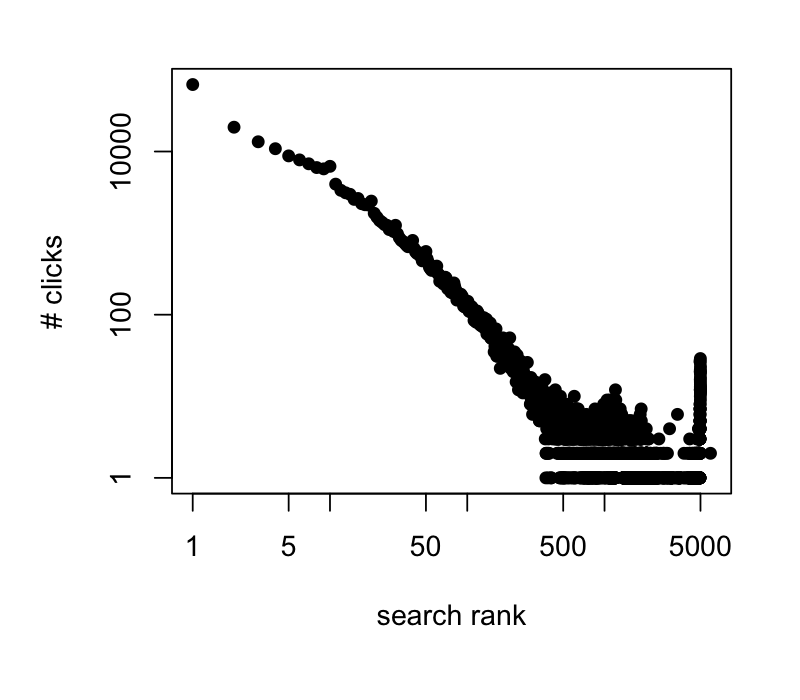
\includegraphics[width=0.5\columnwidth]{../simulations/results/click_distribution.png}
  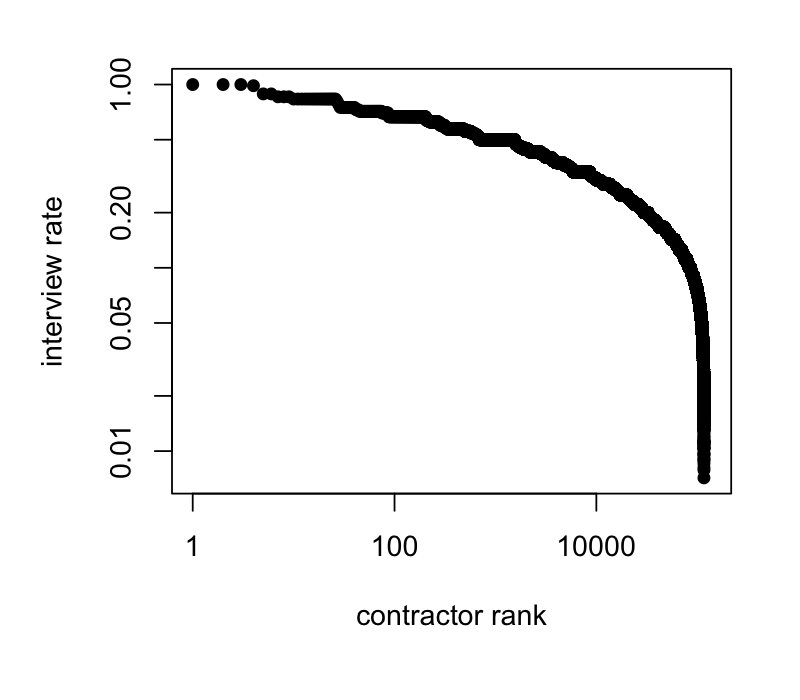
\includegraphics[width=0.5\columnwidth]{../simulations/results/interviewrate_distribution.png}
  \caption{(a) Click distribution per rank position in oDesk
    contractor search. (left) (b) Interview rate at oDesk over a
    period of eight months. (right)}
  \label{fig:clicks}
\end{figure}
To estimate the prominence we use the oDesk contractor search logs
over the period of two weeks of January. The log contains a record for
every click on the search results and each record shows the position
in search and the target contractor profile. In
Figure~\ref{fig:clicks}(a) we plot the click distribution per search
rank position in oDesk contractor search in double logarithmic
scale. The number of clicks drops from approximately 60K in the first
position to 15K in the second and around 200 in the tenth position
(the last position of the first results page). We fitted a Zipfian
distribution to the data and the estimated exponent is 1.35. Our
results are similar to click distribution in traditional web search
\cite{ali2007robust} and indicate dramatic decrease in prominence even
for consecutive positions in search results. In the next paragraph we
show that such distribution is not justified by the contractor merit
distribution.

%\begin{figure}[t]
%  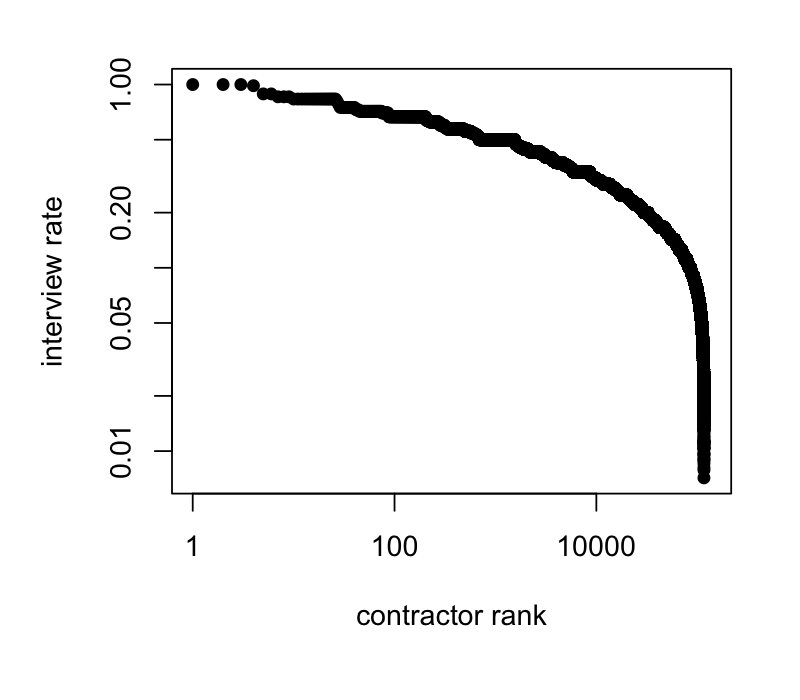
\includegraphics[width=0.4\columnwidth]{../simulations/results/interviewrate_distribution.png}
%  \caption{Interview rate at oDesk over a period of eight months.}
%  \label{fig:interviewrate}
%\end{figure} 

Any constructed measure of merit will be somewhat arbitrary and highly
platform dependent. For oDesk, a reasonable measure of merit is a
constractor's ``success rate'' in seeking jobs. We looked at the job
application history at oDesk over a period of eight months (June 2011
through January 2012) and we calculated each contractor's interview
rate, defined as the ratio of his job applications that evolved into
an interview over his or her total job applications in the period. In
Figure~\ref{fig:clicks}(b) we plot the interview rate distribution in
double logarithmic scale.

By comparing the two Figures~\ref{fig:clicks}(a),(b) we can see how
the search ranking imposes an artificial boost on prominence that is
not justified from an individual's merit.  The gap between the two
distrcibutions shows that there are many contractors who have almost
equal success in convincing with their job applications employers to
setup an interview but receive different prominence through the search
interface.



\section{Empirical mechanism comparison}
\label{sec:expr-comparison}
In this section we compare the algorithms that we have presented in
terms of runtime performance and the satisfaction of the exact
proportion condition. For our comparison we use synthetic data that
capture different scenarios for the budget distribution across the
population. In all of the scenarios we assume that the prominence in
different rank positions follow the Zipfian distribution that we
observed in Section~\ref{sec:expr-odesk}.

\subsubsection{Runtime performance}
\label{sec:expr-runtime}

We compare the runtime performance of the EP algorithm
(Algorithm~\ref{alg:find-equitable}) and two different variations of
the RT algorithm (Algorithm~\ref{alg:tontine}). In the first
variation, called \emph{naive} RT, we renormalize the weights of
individuals after each assignment of an individual to a position. In
the second variation, called \emph{tree-based} RT, we leverage the
tree structure described in Section~\ref{sec:tontine}.

The comparison setting is the following. For different sizes $n$ of
the population we assign merit values to the individuals using uniform
sampling in the range $[0,1]$ and we set the prominence of each of the
$n$ search positions to follow a Zipfian distribution with exponent
$1.35$. We do not report results for other distributions in this
section, since our experiments showed that the distribution types have
negligible impact on the algorithms performance. For each value of $n$
we ran all of the three algorithms and we measured the runtime in
seconds. 
\begin{figure}[t]
  \centering
  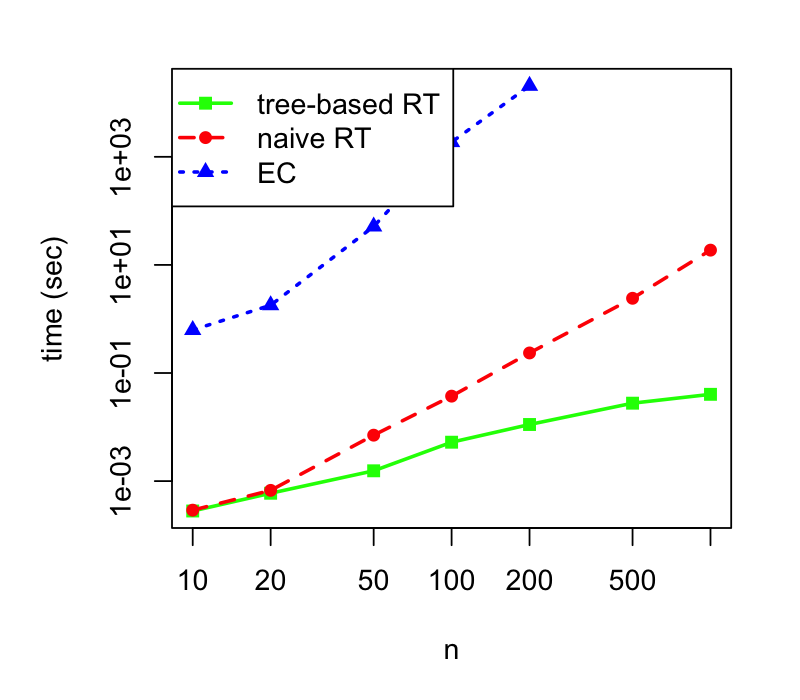
\includegraphics[width=0.6\columnwidth]{../simulations/results/performance.png}
  \caption{Runtime comparison of the three different assignment
    algorithms.}
  \label{fig:runtime}
\end{figure} 
We report the results in Figure~\ref{fig:runtime}. The x-axis shows
the number of individuals in the population and the y-axis shows the
time in logarithmic scale. There are three lines in the plot and each
line looks at a different algorithm. The solid line looks at the
tree-based RT, the dashed line looks at the naive RT, and the dotted
line looks at the EP algorithm. The closer a line to the x-axis the
better the algorithm. We observe that tree-based can rank up to $1000$
individuals in much less than a second. The tree-based RT achieves
also significantly faster runtime than the naive RT, which shows the
benefits of the tree structure we use to expedite sampling. As far as
the EP algorithm is concerned, we did not to run it for $n$ greater
than $200$, since the $6$ hours it took to rank $200$ individuals
convinced us that it cannot be used in practice. To summarize, the
tree-based RT algorithm is much faster than the other algorithms and
its runtime make it practical for real-world scenarios.


\subsubsection{Equitable prominence approximation}
\label{sec:expr-approximation}
Although we showed that the RT algorithm is fast enough to be applied
to real-world scenarios, we have not still evaluated its impact on the
prominence allocation problem. Recall that the algorithm does not
yield equitable prominence in the general case as the EP algorithm
does. However, the RT algorithm ensures continuity and monotonicity in
merit, two properties that are missing from the vanilla assortative
ranking.

In this section we compare the assortative ranking, and the rankings
obtained from the RT and the EP algorithms in terms of their
prominence allocation for different merit distributions. To obtain
different merit distribution we sample from the Pareto distribution
with different $\alpha$ parameters. Recall that when $\alpha$ is
large, the Pareto distribution approaches the Dirac distribution at
point $1$. That means, that all of the sampled individuals' merits
will be almost equal to $1$. As the value of parameter $\alpha$
decreases, the merit values get spreaded out and finally the Pareto
distribution becomes skewed. That is, it yields few individuals with
extremely high merit values and many individuals with low merit
values. To evaluate the effect of the different rankings across the
spectrum of different Pareto distributions we used the following
values for $\alpha$: $100$, $10$, $5$, $1$ and $0.5$. Although
we use different merit distributions,we use in every case a Zipfian
distribution with exponent $1.35$ to model the prominence distribution
over the search positions.

For each distribution of merits we ran each of the algorithms $m$
times to obtain the average prominence for each individual $\bar{v_i}$
across the $m$ runs\footnote{We did not actually run the EP algorithm,
  since it was theoretically shown to achieve equitable prominence
  allocation}. To evaluate the success of the algorithms in achieving
equitable prominence allocation, we use the root mean square error
(RMSE) defined as:
\[
\sqrt{\frac{\sum_{i=1}^n\left(\frac{b_i}{\sum_{j=1}^n
        b_j}-\frac{\bar{v_i}}{\sum_{j=1}^n \bar{v_j}}\right)^2}{n}}
\]
\begin{figure}[t]
  \centering
  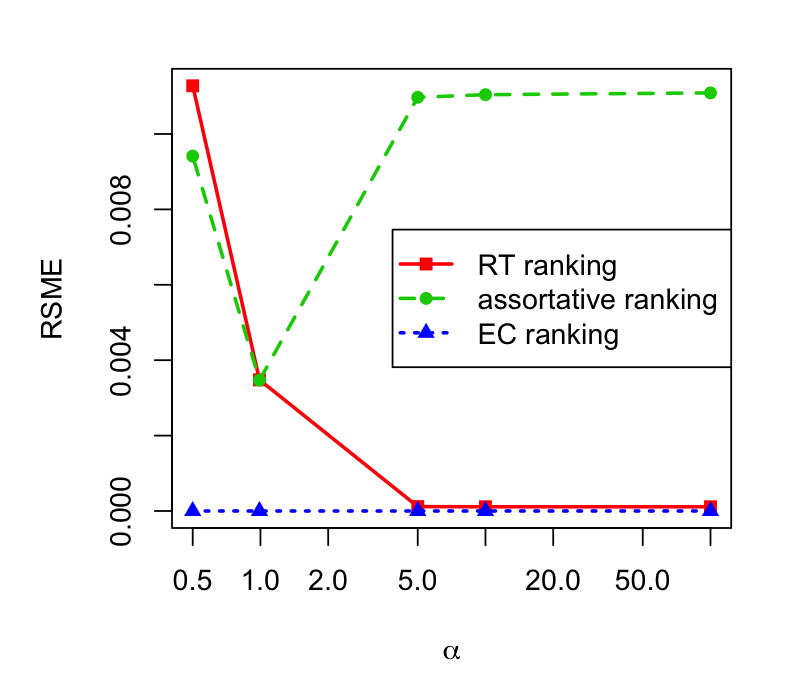
\includegraphics[width=0.6\columnwidth]{../simulations/results/approximation.png}
  \caption{RMSE in the approximation of equitable allocation for the
    three different ranking approaches. The contractor merits are
    randomly sampled from a Pareto distribution with parameter $\alpha$.}
  \label{fig:approximation}
\end{figure} 
We plot the results in Figure~\ref{fig:approximation} for
$m=1000$. The x-axis shows the value of the Pareto distribution
parameter and the y-axis shows the RSME. There are three lines in the
plot and each looks at a different ranking approach. The solid line
looks at the RT ranking, the dashed line looks at the assortative
ranking and the dotted line looks at the estimated EP ranking. Note
that RMSE is 0 for the EP ranking, since the EP algorithm is
guaranteed to achieve equitable prominence allocation for any merit
distribution. The assortative distribution has small RMSE for low
values of $\alpha$, because in these case the merit distribution
become similar to the Zipfian prominence distribution. However, the
real-world data in Section~\ref{sec:expr-odesk} showed that these
distributions are not similar. As $\alpha$ increases the assortative
ranking yields significantly greater RMSE that the other ranking
approaches. Finally, note that the RT ranking yields RMSE that is very
close to $0$ for a wide range of $\alpha$ values. The RMSE increases
for small values of $\alpha$ that yield distributions that were not
observed in the oDesk dataset. Thus, we can conclude that the RT
algorithm yields prominence that is close to the equitable allocation
for practical cases. This result combined with its ability to scale
make it an attractive option for real-world applications.



\section{Conclusions and Future Work} 

In this paper, we have defined a problem common to two-sided
platforms, which is the allocation of visbility to platform
participants. We have also demonstrated the problem using data from an
actual online labor market. We described the relationship of this
problem to the classic economic assignment problem and proposed a
number of additional criteria for evaluating assignment mechanisms that
are relevant in the platform/repeated assignment setting that we are
focused on. We show that it is possible to create an assignment that
satisfied the exact proportion criterion, using our RC
algorithm, but also show that the standard solution is infeasible for
web-scale applications.  As a substitute, we proposed an algorithm RT
that has some nice properties that make it well-suited for
applications, including reasonable approximation to the equity
criterion. However, we hope that future work might demonstrate how
this algorithm could be modified, perhaps by having some ``memory'' of
past allocations to yield assignments that are equitable in
expectation.



\bibliographystyle{aer}
\bibliography{visibility_allocation.bib}

\end{document}
